\chapter{Options for General Video Game Playing}

Options have previously mostly been used in specific cases and for relatively
simple problems. To specify the problem domain, this chapter will cover how a
game is defined in VGDL and how it is observed by the game playing algorithm.
Furthermore, we will explain what options mean in the context of general video
game playing and what we have done to create a set of options that can be used
in any game. Lastly, this chapter explains what is needed to use SMDP Q-learning
on the domain of general video game playing.

\section{Toy Problem}

As described in the background section, the foundation of a game lies in two
specifications. The game dynamics, and levels. The game dynamics are typically
the same for each level and do not change over the course of a game. Levels
define the layout of the game. Each level is different and typically the last
level of a game is harder than the first level.

In VGDL, the game description defines the game dynamics. Each game has one game
description file, which describes the game sprites and their interaction with
each other. The levels are defined in separate level files and define the layout
of the screen.

In this section, we introduce our test game \emph{prey}. We created this game
for testing the learning capacities of the algorithm. Furthermore, this section
contains an in-depth explanation of the VGDL. The game aims to be simple to
understand and easy to win. It should be possible to see any improvement an
algorithm could achieve as well. We chose the \emph{predator \& prey} game, in
which the player is a predator, that should catch its prey (an NPC) by walking
into it. We decided to have three types of prey, one that never moves, one that
moves once in 10 turns and one that moves once in 2 turns. This section
describes how the game is made in VGDL and how a GVGAI agent can interact with
it.

\lstinputlisting[basicstyle=\footnotesize, frame=tb, xleftmargin=.1\textwidth, %
xrightmargin=.1\textwidth, caption=prey.txt, label=lst:preytxt, float=t]%
{../examples/gridphysics/prey.txt}

\begin{minipage}[t]{.4\textwidth}
	\lstset{
		caption=Prey level 1, 
		label=lst:prey1,
		basicstyle=\footnotesize, frame=tb,
		xleftmargin=.1\textwidth, xrightmargin=.1\textwidth
	}
	\begin{lstlisting}
wwwwwww
wA    w
w     w
w     w
w    Iw
wwwwwww
	\end{lstlisting}
\end{minipage}
\begin{minipage}[t]{.5\textwidth}
	\lstset{
		caption=Prey level 2,
		label=lst:prey2,
		basicstyle=\footnotesize, frame=tb,
		xleftmargin=.1\textwidth, xrightmargin=.1\textwidth
	}
	\begin{lstlisting}
wwwwwwwwwwwww
wA     w    w
w      w    w
w      w    w
w wwwwww    w
w           w
w           w
w           w
w           w
w           w
w           w
w       wwwww
w          Iw
wwwwwwwwwwwww
	\end{lstlisting}
\end{minipage}

The code in Listing \ref{lst:preytxt} contains the game description. Lines 2 to
8 describe the available sprites. There are two sprites in the game, which are
both \texttt{movable}: the avatar (predator) and the monster (prey).  The avatar
is of type \texttt{MovingAvatar}, which means that the player has four possible
actions (up, right, down, left). The prey has three instantiations, all of the
type \texttt{RandomNPC}, which is an NPC that moves about in random directions:
the \texttt{inactivePrey}, which only moves every 3000 steps (which is more than
the timeout explained shortly, so it never moves); the \texttt{slowPrey} which
moves once every 10 steps, and the \texttt{fastPrey} which moves once every 2
steps.  By default, the \texttt{MovingAvatar} can move once in each time step.

Lines 10 to 14 describe the level mapping. These characters can be used in the
level description files, to show where the sprites spawn. 

In the interaction set, Line 17 means that if the prey walks into the avatar (or
vice versa) this will kill the prey, and the player will get a score increase of
one point. Line 18 dictates that no \texttt{movable} sprite can walk through
walls.

Lastly, in the termination set, line 21 shows that the player wins when there
are no more sprites of the type \texttt{prey}, and line 22 shows that the player
loses after 100 time steps.

Listing \ref{lst:prey1} shows a simple level description. This level is
surrounded with walls and contains one avatar and one inactive prey. 
The game can be used to test the functionality of an algorithm. The first level
is very simple and is only lost when the agent is not able to find the prey
within the time limit of 100 time steps, which is unlikely. A learning
algorithm should, however be able to improve the number of time steps it needs
to find the prey. The minimum number of time steps to win the game in the first
level, taking the optimal route, is six. Listing \ref{lst:prey2} defines the
second level, which is more complex. The agent has to plan a route around the
walls and the prey is further away. We chose to still use the inactive prey in
this case, because then we know that the minimum number of time steps needed to
win is always twenty.

An agent that starts playing \textit{prey} in the GVGAI framework, observes the
world as defined by the level description. It knows where all the sprites are,
but it does not know in advance how these sprites interact. The other relevant
observations for this game are the avatar's direction and speed and the game
tick. When an algorithm plays the game, it has a limited amount of time to
choose an action, based on the observation. It can access a \emph{forward
model} that simulates the next state for applying a certain action. The forward
model can be polled infinitely, but an action has to be returned by the
algorithm within the action time.

\section{Option Set}
Human game players consider subgoals when they are playing a game. Some of these
subgoals are game-independent. For example, in each game where a player has a
movable avatar the player can decide it wants to go somewhere or avoid
something. These decisions manifest themselves as subgoals, which are formalized
in this section in a set of options.  

In this section, we describe our set of options which can be used in any game
with a movable avatar and provides the means to achieve the subgoals mentioned
above. Note that a more specific set of options can be created when the
algorithm should be tailored to only one type of games and similarly: options
can be added and removed from the set easily. The following options are
designed and will be used in the experiments in chapter \ref{sec:experiments}:

\begin{itemize}
	\item \texttt{ActionOption} executes a specific action once and then
		stops.
		\begin{itemize}
			\item Invocation: the option is invoked with an action.
			\item Subtypes: one subtype is created for each action in action set
				$A$.
			\item Initiation set: any state $s_t$
			\item Termination set: any state $s_{t+1}$
			\item Policy: apply the action corresponding to the subtype.
		\end{itemize}
	\item \texttt{AvoidNearestNpcOption} makes the agent avoid the nearest NPC
		\begin{itemize}
			\item Invocation: this option has no invocation arguments
			\item Subtypes: this option has no subtypes
			\item Initiation set: any state $s_t$ that has an NPC on the
				observation grid
			\item Termination set: any state $s_{t+1}$
			\item Policy: apply the action that moves away from the NPC. This
				option ignores walls.
		\end{itemize}
	\item \texttt{GoNearMovableOption} makes the agent walk towards a
		movable game sprite (defined as movable by the VGDL) and stops when it
		is within a certain range of the movable
		\begin{itemize}
			\item Invocation: this option is invoked on a movable sprite in the
				observation grid.
			\item Subtypes: the subtype corresponds to the type of the sprite
				this option follows.
			\item Initiation set: any state $s_t$ with the goal sprite in the observation grid
			\item Termination set: any state $s_{t+n}$ in which the path from
				the avatar to the goal sprite is smaller than 3 actions and all the states
				$s_{t+n}$ that do not contain the goal sprite.
			\
			\item Policy: apply the A Star action that leads to the goal sprite.
		\end{itemize}
	\item \texttt{GoToMovableOption} makes the agent walk towards a
		movable until its location is the same as that of the movable
		\begin{itemize}
			\item Invocation: this option is invoked on a movable sprite in the
				observation grid.
			\item Subtypes: the subtype corresponds to the type of the sprite
				this option follows.
			\item Initiation set: any state $s_t$ with the goal sprite in the
				observation grid
			\item Termination set: any state $s_{t+n}$ in which the goal sprite
				location is the same as the avatar location and all the states
				$s_{t+n}$ that do not contain the goal sprite.
			\item Policy: apply the A Star action that leads to the goal sprite.
		\end{itemize}
	\item \texttt{GoToNearestSpriteOfType} makes the agent walk to the nearest
		sprite of a specified type
		\begin{itemize}
			\item Invocation: the option is invoked with a sprite type.
			\item Subtypes: the subtype corresponds to the invocation sprite type.
			\item Initiation set: any state $s_t$ that has the sprite type
				corresponding to the subtype in its observation grid
			\item Termination set: any state $s_{t+1}$ where the location of the
				avatar is the same as a sprite with a type corresponding to
				the subtype, or any state that has no sprites of this option's
				subtype.
			\item Policy: apply the A Star action that leads to the nearest
				sprite of this option's subtype.
		\end{itemize}
	\item \texttt{GoToPositionOption} makes the agent walk to a specific
		position.
		\begin{itemize}
			\item Invocation: the option is either invoked on a specific goal
				position in the grid or with a static sprite.
			\item Subtypes: if the option was invoked on a specific sprite, the
				subtype is that sprite's type.
			\item Initiation set: any state $s_t$. If the goal is a sprite, this
				sprite has to be in the observation grid.
			\item Termination set: any state $s_{t+n}$ in which the avatar
				location is the same as the goal location.
			\item Policy: apply the A Star action that leads to the goal
				location.
		\end{itemize}
	\item \texttt{WaitAndShootOption} waits until an NPC is in a specific location and
		then uses its weapon.
		\begin{itemize}
			\item Invocation: the option is invoked with a distance from which
				the avatar will use his weapon.
			\item Subtypes: a subtype is created for each invocation distance
			\item Initiation set: any state $s_t$
			\item Termination set: any state $s_{t+n}$ in which the agent has
				used his weapon
			\item Policy: do nothing until an NPC moves into a given distance,
				then use the weapon (action \textsc{use})
		\end{itemize}
\end{itemize}

\begin{figure}
	\centering
	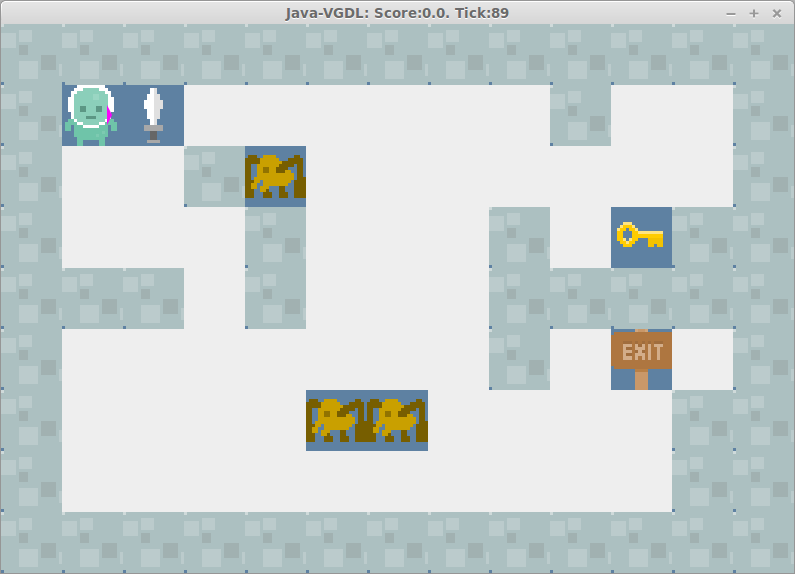
\includegraphics[width=.6\textwidth]{includes/zelda}
	\caption{Visual representation of the game \textit{zelda}.}
	\label{fig:zelda}
\end{figure}

For each option type, a subtype per visible sprite type is created during the
game. For each sprite, an option instance of its corresponding subtype is
created. For example, the game \textit{zelda}, as seen in Figure \ref{fig:zelda},
contains three different sprite types (excluding the avatar and walls);
monsters, a key and a portal. The first level contains three monsters, one key
and one portal, and the aim of the game is to collect the key and walk towards
the portal without being killed by the monsters. The score is increased by 1 if
a monster is killed (i.e., its sprite is on the same location as the sword
sprite) if the key is picked up, and when the game is won.
\texttt{GoToMovableOption} and \texttt{GoNearMovableOptions} are created for
each of the three monsters and for the key. A \texttt{GoToPositionOption} is
created for the portal.  One \texttt{GoToNearestSpriteOfType} is created per
sprite type. One \texttt{WaitAndShootOption} is created for the monsters, and
one \texttt{AvoidNearestNpc\-Option} is created. This set of options is $O$, as
defined in Section \ref{subsec:options}. In a state where, for example, all the
monsters are dead, the possible option set $\mathbf{p}_s$ does not contain the
\texttt{AvoidNearestNpcOption} and \texttt{GoToMovableOption}s and
\texttt{GoNearMovableOption}s for the monsters.

The role of the \texttt{GoTo\ldots} options is to enable the avatar to reach the
key and the portal. The \texttt{GoNear\ldots} options can be used to motivate
the avatar to go near a monster, because if the avatar uses its sword (or the
\texttt{WaitAndShootOptions} on a monster, the game can be won with a higher
score. The \texttt{AvoidNearestNpcOption} functions to save the avatar from
monsters that come too close. If the algorithms encounters a game in which these
options can not lead to winning the game, it can use the \texttt{ActionOptions},
that function the same as normal actions.

The \texttt{GoTo\ldots} and \texttt{GoNear\ldots} options utilize an adaptation
of the A Star algorithm to plan their routes. An adaptation is needed, because
at the beginning of the game there is no knowledge of which sprites are
traversable by the avatar and which are not. Therefore, during every move that
is simulated by the agent, the A Star module has to update its beliefs about the
location of walls and other blocking objects. This is accomplished by comparing
the movement the avatar wanted to make to the movement that was actually made in
game. If the avatar did not move, it is assumed that all the sprites on the
location the avatar should have arrived in are blocking sprites. A Star keeps a
\emph{wall score} for each sprite type. When a sprite blocks the avatar, its
wall score is increased by one. Additionally, when a sprite kills the avatar,
its wall score is increased by 100, in order to prevent the avatar from walking
into killing sprites.  Traditionally the A Star's heuristic uses the distance
between two points. Our A Star adaptation adds the wall score of the goal
location to this heuristic, encouraging the algorithm to take paths with a lower
wall score. This method enables A Star to try to traverse paths that were
unavailable earlier, while preferring safe and easily traversable paths. For
example in \textit{zelda}, a door is closed until a key is picked up. Our A Star
version will still be able to plan a path to the door once the key is picked up,
winning the game.


\section{SMDP Q-learning for General Video Game Playing}
\label{subsec:smdp-qlearning-gvgp}

This option set is used by the SMDP Q-learning algorithm. The algorithm was
adjusted to work as an anytime algorithm in the GVGAI competition framework.
Our implementation uses interruption when applying actions to the game, but not
during planning. This way, the algorithm can identify options that are good
during planning, but will not follow then in dangerous situations that have not
been encountered during planning. This is advantageous in our situation, where
there is only a short amount of planning time before an action has to be chosen.
Furthermore, because of the time limitation we added a maximum search depth $d$
to the algorithm that limits exploration to the direct surroundings of a state.

\begin{algorithm}[h]
	\caption{$\mathsf{SMDP~Q-learning}(Q, O, s, t, d, o)$}
	\label{alg:ql}
	\begin{algorithmic}[1]
		\State $\mathbf{i} \gets \emptyset$ \Comment{$i_o$ counts the number of steps an option has been used}
		\While {$time\_taken < t$} \label{alg:ql:smainloop}
			\State $s' \gets s$ \label{alg:ql:copys} \Comment{Copy the initial state}
			\If{$s' \in \beta(o)$} \label{alg:ql:sno} \Comment{if option stops in state $s'$}
				\State $o \gets \mathsf{epsilon\_greedy\_option}(s', Q, O)$ 
					\Comment{Get epsilon greedy option}
				\State $i_o \gets 0$ \Comment{reset step counter $i_o$}
			\EndIf \label{alg:ql:eno}
			%\For{$depth$ \textbf{in} $\left{0 \ldots d\right}$}
			\For{$depth$ \textbf{in} $\left\{ 0 \ldots d \right\} $} \label{alg:ql:sfor}
				\State $a \gets \mathsf{get\_action}(o, s')$ 
					\Comment{get action from $o$}
				\State $(s', r) \gets \mathsf{apply\_action}(s', a)$ \label{alg:ql:apply}
					\Comment{set $s'$ to new state, get reward $r$}
				\State $\mathsf{update\_option}(Q, o, s', r, \mathbf{i})$ 
					\Comment{Algorithm \ref{alg:update}}
				\If{$s' \in \beta(o)$} 
					\Comment{Same as lines \ref{alg:ql:sno} to \ref{alg:ql:eno}}
					\State $o \gets \mathsf{epsilon\_greedy\_option}(s', Q, O)$ 
					\State $i_o \gets 0$
				\EndIf
			\EndFor \label{alg:ql:efor}
		\EndWhile \label{alg:ql:emainloop}
		\State \Return{$\mathsf{get\_action}(\mathsf{greedy\_option}(s, Q, O), s)$}
	\end{algorithmic}
\end{algorithm}
\begin{algorithm}[h]
	\caption{$\mathsf{update\_option}(Q, o, s, r, \mathbf{i})$}
	\label{alg:update}
	\begin{algorithmic}[1]
		\State $i_o \gets i_o + 1$ \Comment{Increase this option's step count by 1}
		\State $o_r \gets o_r + \gamma^{i_o} r;$
			\Comment{Change this option's discounted reward}
		\If{$s \in \beta(o)$} \Comment{if option stops in state $s$}
			\State $\mathsf{update\_Q}(o, s, o_r, i_o)$ \Comment{Equation
			\ref{eq:smdp-qlearning} }
		\EndIf
	\end{algorithmic}
\end{algorithm}

Our implementation of the algorithm is formalized in Algorithm \ref{alg:ql}. We
initialize Q-learning with the table $Q$ (empty in the first game), a predefined
option set $O$, the current state $s$, a time limit $t$, the maximum search
depth $d$ and the currently followed option $o$ (for the first iteration of a
game, initialize $o$ to any finished option). The algorithm starts with a loop
that keeps running as long as the maximum time $t$ is not surpassed, from line
\ref{alg:ql:smainloop} to \ref{alg:ql:emainloop}. In line \ref{alg:ql:copys},
the initial state $s$ is copied to $s'$, for mutation in the inner loop. Then,
in lines \ref{alg:ql:sno} to \ref{alg:ql:eno}, the algorithm checks if a new
option is needed. If the currently used option $o$ is finished, meaning that
state $s'$ is in its termination set $\beta(o)$, a new option is chosen with an
epsilon greedy policy. 

Then, from lines \ref{alg:ql:sfor} to \ref{alg:ql:efor} the option provides an
action, which is applied to the simulator in line \ref{alg:ql:apply}.
Afterwards, the option's return, and possibly the Q-table, are updated by the
function \textsf{update\_option} as displayed in Algorithm \ref{alg:update}.
Finally, if the option is finished, a new option is selected with the
epsilon greedy policy. The inner loop keeps restarting until a maximum depth is
reached, after which the outer loop restarts from the initial state.

Algorithm \ref{alg:update} describes how our \textsf{update\_option}
function works: first the step counter $i_o$ is increased. Secondly, the
cumulative discounted reward is altered. If the option is finished, $Q$ is
updated using Equation \ref{eq:smdp-qlearning} (note that in the equation the
cumulative reward $o_r$ is $r$, and step counter $i_o$ is $k$). Note that by
keeping the discounted option value, we do not have to save a reward history
for the options.

By repeatedly applying an epsilon greedy option's actions to the game, the
Q-values of promising options should quickly converge to indicate which option
should be chosen in which game state. When the time runs out, the algorithm
returns the action chosen by the greedy option, which is the best option for
state $s$ at that moment. After the action has been applied, the algorithm is
restarted with the new state. Chapter \ref{sec:experiments} describes the
experiments we have done with this implementation of SMDP Q-learning.

SMDP Q-learning is a robust algorithm that is theoretically able to learn the
best option for each of the states in a game. The problem, however, is that the
algorithm has a slow learning process. Furthermore, Q-learning requires that the
algorithm saves all the states that were visited, which means that the Q-table
can quickly grow to a size that is infeasible. Therefore, we propose a new
algorithm that combines the advantages of using options with using Monte Carlo
tree search.
